\section*{Supplementary material}


\subsection*{Proofs}

Full proof of Proposition 1.
\begin{proof}
We build the proof on the result of Beck and Wilson~\cite{beck2007proactive}, who established a lower bound for RCPSPs that do not account for resource unavailability. The core argument relies on the ability to represent RCPSP constraints as Positive Precedence Expressions (PPEs).
Specifically, the constraints of an RCPSP can be expressed as a conjunction of PPEs~(\cite{beck2007proactive}):
\begin{enumerate}
    \item \textbf{Precedence Constraints (\( \phi \))}: Precedence relationships between activities \( a_i \) and \( a_j \) are represented as primitive precedence expressions \( \texttt{before}(i, j) \). Let \( \phi \) denote the conjunction of all such precedence constraints.

    \item \textbf{Resource Constraints (\( \psi \))}: Resource constraints can be represented using forbidden sets. A forbidden set \( H \subseteq \mathcal{A} \) consists of activities whose simultaneous execution exceeds the capacity of a resource \( r \), $C_r$. Resource constraints are satisfied if, for all \( H \in F \), there exist two activities \( a_i, a_j \in H \) such that \( \texttt{before}(i, j) \) holds. This is expressed as:
    \[
    \psi = \bigwedge_{H \in F} \bigvee_{a_i, a_j \in H, i \neq j} \texttt{before}(i, j).
    \]
\end{enumerate} Combining these, the constraints of an RCPSP are represented as \( \phi \wedge \psi \), which is a conjunction of PPEs. In BPSP, resource unavailability introduces additional constraints:
each resource \( r \) has an availability calendar \( v_{r,t} \), where \( v_{r,t} = 1 \) if \( r \) is available at time \( t \), and \( 0 \) otherwise.
To incorporate resource unavailability, we redefine and extend the notion of forbidden sets:
\begin{enumerate}
    \item Capacity forbidden sets \( H \) are defined as in RCPSPs, representing sets of activities whose simultaneous execution exceeds the capacity of a resource \( r \).
    \item For resource unavailability, we extend \(H\) with additional constraints for each resource \( r \) and time \( t \) where \( v_{r,t} = 0 \). The extended forbidden sets, denoted $H'$, ensure that no activities requiring \( r \) overlap during unavailable periods.
\end{enumerate} The resource constraints with unavailability can then be expressed as:
\[
\psi_u = \bigwedge_{H' \in F'} \bigvee_{a_i, a_j \in H', i \neq j} \texttt{before}(i, j),
\]
where \( F' \) is the extended set of forbidden sets that includes both capacity constraints and unavailability constraints.

The combined constraints for BPSP, including resource unavailability, can now be expressed as:
\[
\phi \wedge \psi_u,
\]
where \( \phi \) represents precedence constraints, and \( \psi_u \) represents resource constraints, including unavailability. Each component is a conjunction of PPEs, ensuring that the overall problem retains the PPE structure.

Since BPSP constraints can be expressed as a conjunction of PPEs, the results from~\cite{beck2007proactive} apply, and \( q_U \) provides a lower bound on the stochastic makespan.
\end{proof} 


\begin{figure*}[t]
\centering
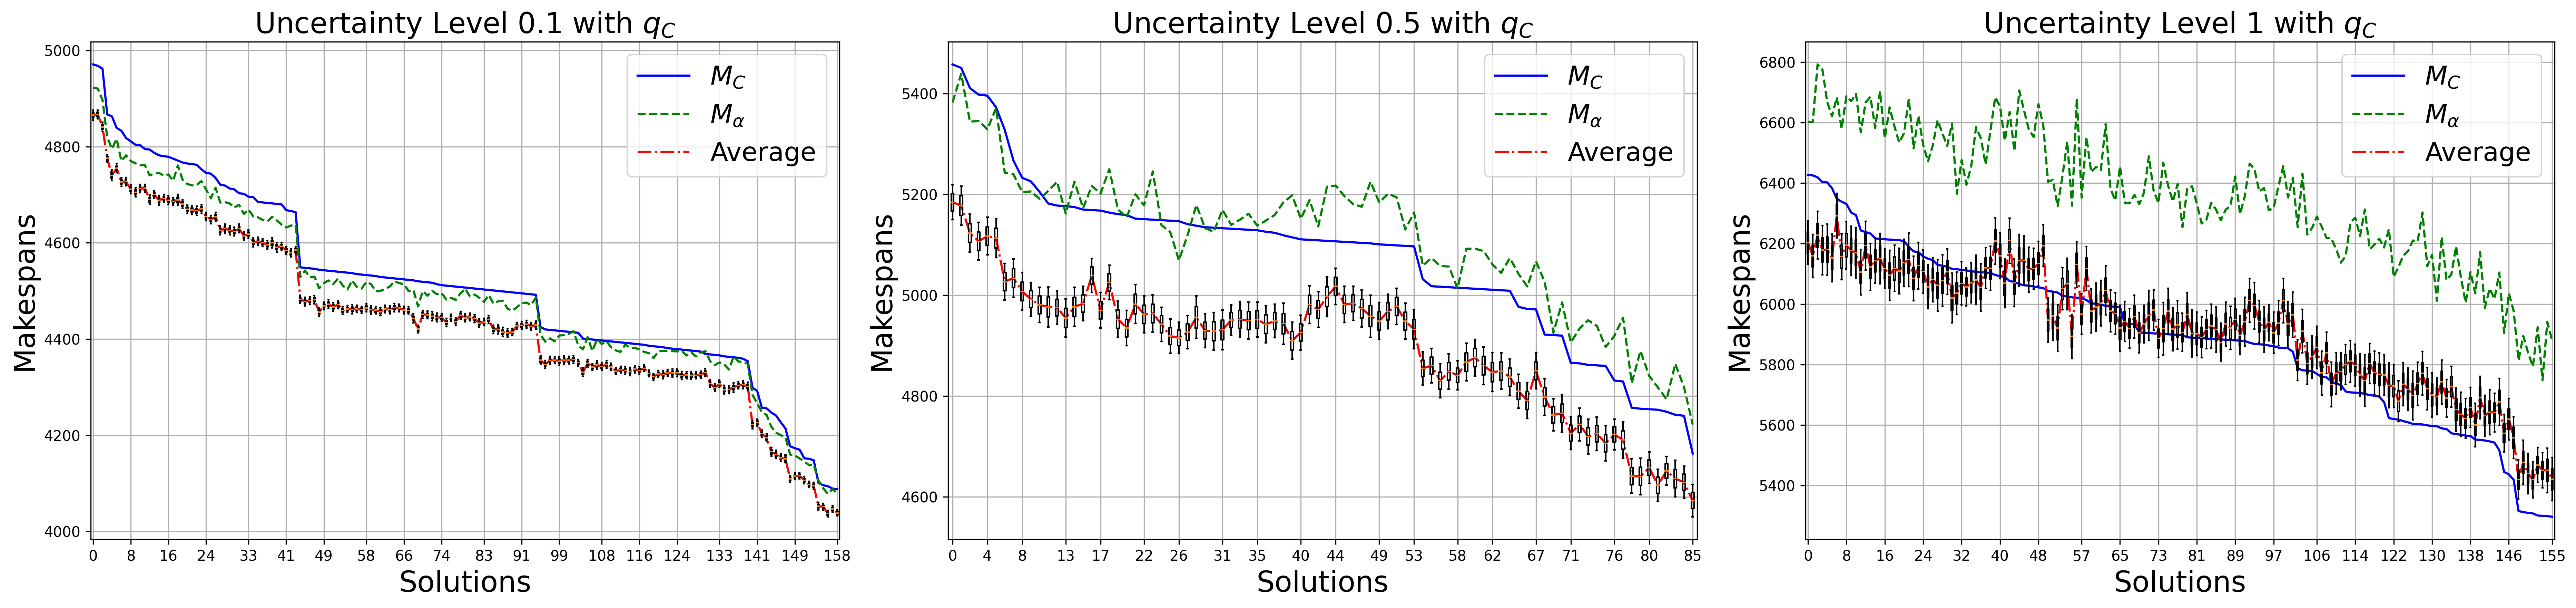
\includegraphics[width=\textwidth]{images/q3_results.png}
\caption{Comparison of all $M_C$ solutions returned by the CP solver with $q_C$, along with their corresponding $M_{\alpha}$ values and the \emph{Mean} computed over 1,000 simulations, for the synthetic \act{medium} problem without calendars for each level of uncertainty ($0.1, 0.5, 1.0$). }
\label{fig:q3_results}
\end{figure*}

\begin{figure*}[t]
\centering
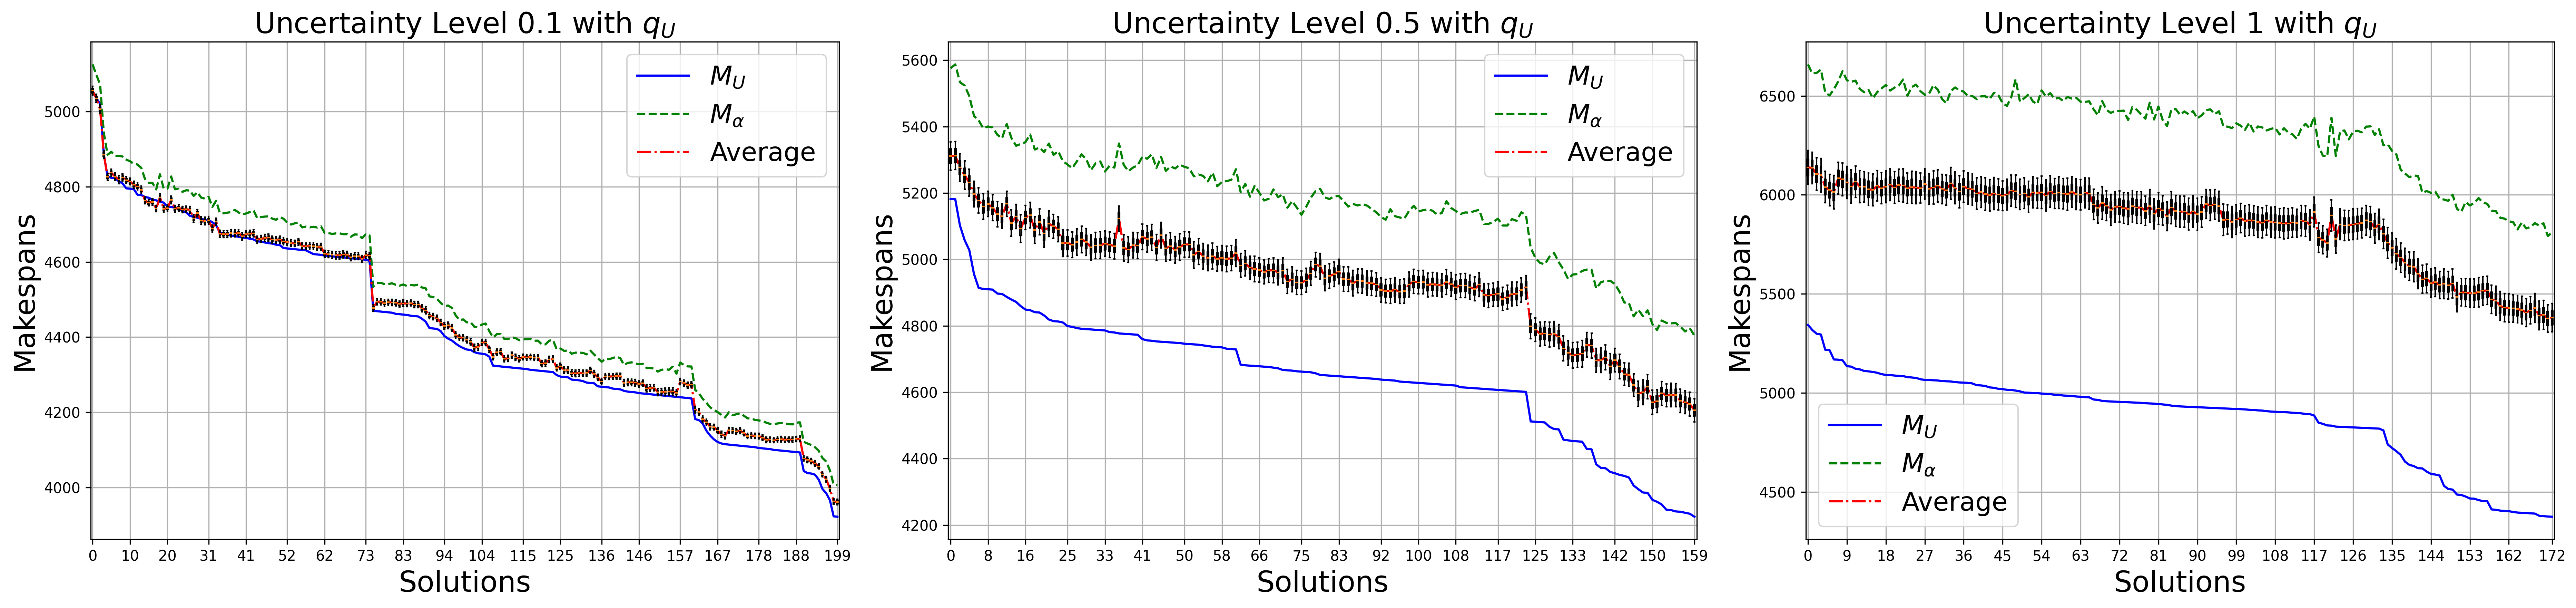
\includegraphics[width=\textwidth]{images/q1_results.png}
\caption{Comparison of all $M_C$ solutions returned by the CP solver with $q_U$, along with their corresponding $M_{\alpha}$ values and the \emph{Mean} computed over 1,000 simulations, for the synthetic \act{medium} problem without calendars for each level of uncertainty ($0.1, 0.5, 1.0$).}
\label{fig:q1_results}
\end{figure*}




\begin{table*}[h]
\centering
\scalebox{0.95}{
\begin{tabular}{l@{\hskip 0.05in}c@{\hskip 0.05in}c@{\hskip 0.07in}c@{\hskip 0.05in}c@{\hskip 0.05in}c@{\hskip 0.05in}c@{\hskip 0.05in}c@{\hskip 0.05in}c@{\hskip 0.05in}c@{\hskip 0.05in}c@{\hskip 0.04in}c@{\hskip 0.05in}c@{\hskip 0.05in}c@{\hskip 0.05in}c@{\hskip 0.05in}c@{\hskip 0.04in}}
\toprule
\textbf{Size} & \textbf{Unc.} & \textbf{$q_{C}$} & \multicolumn{5}{c}{Sets} & \multicolumn{5}{c}{Calendars} &
 \\
& \textbf{Level} & & $M^*_{C}$ & $M^*_{alpha}$ & $\mu^*_{\alpha}$ & $\sigma^*_{\alpha}$ &  NP & $M^*_{C}$ & $M^*_{alpha}$ & $\mu^*_{\alpha}$ & $\sigma^*_{\alpha}$ & NP \\
\midrule
\multirow{3}{*}{10 X 10} & 0.1 & 0.623 & 1264 & 1267.117 & 1247.123 & 12.605 & 1.00 & 6306 & 6318.929 & 6311.387 & 34.791 & 1.00 \\
  & 0.5 & 0.612 & 1412 & 1461.083 & 1375.390 & 55.351 & 1.03 & 6522 & 6557.094 & 6530.092 & 309.877 & 1.00 \\
  & 1 & 0.582 & 1606 & 1818.667 & 1634.942 & 118.814 & 1.13 & 10592 & 12012.313 & 10405.540 & 1254.506 & 1.13\\
\midrule

\multirow{3}{*}{20 X 15} & 0.1 & 0.617 & 857 & 984.894 & 920.013 & 41.663 & 1.15 & 10532 & 10544.230 & 10550.919 & 181.384 & 1.00\\
  & 0.5 & 0.631 & 876 & 985.649 & 917.516 & 40.973 & 1.12 & 10845 & 10880.421 & 10884.615 & 261.896 & 1.00\\
  & 1 & 0.592 & 870 & 985.131 & 911.594 & 42.759 & 1.13 & 10584 & 11672.917 & 10672.633 & 340.185 & 1.10\\
  \midrule

 \multirow{3}{*}{20 X 20} & 0.1 & 0.726 & 4088 & 4079.711 & 4041.146 & 24.760 & 0.99 & 17305 & 17310.267 & 17305.266 & 136.515 & 1.00\\
  & 0.5 & 0.697 & 4686 & 4810.094 & 4600.222 & 121.340 & 1.03 & 21413 & 23461.411 & 22547.239 & 790.885 & 1.10\\
  & 1 & 0.657 & 5297 & 5836.450 & 5442.214 & 235.606 & 1.10 & 22802 & 27096.049 & 24824.725 & 1415.784 & 1.10\\
\midrule


\multirow{3}{*}{30 X 15} & 0.1 &  0.680& 5014 & 4987.340 & 4931.863 & 32.466 & 0.99 & 21701 & 21717.042 & 21711.987 & 4.136 &  1.00 \\
  & 0.5 & 0.657 & 5708 & 5792.257 & 5567.154 & 143.244 & 1.01 &  23417 & 24833.082 & 23561.022 & 464.668 & 1.06 \\
  & 1 & 0.724 & 6324 & 6854.744 & 6459.147 & 246.865 & 1.08 & 34605 & 34605.057 & 32865.581 & 837.235 & 1.00\\
\midrule

\multirow{3}{*}{40 X 20} & 0.1 & 0.653 & 6716 & 6689.988 & 6628.501 & 36.241 & 0.99 & 33950 & 35390.976 & 34151.698 & 516.134 & 1.04 \\
  & 0.5 & 0.690 & 8569 & 8524.441 & 8258.515 & 159.984 & 0.99 & 32384 & 35267.634 & 33782.977 & 1389.356 & 1.09 \\
  & 1 &  0.648 & 8966 & 9622.562 & 9167.436 & 289.895 & 1.07 & 35523 & 43038.499 & 40990.318 & 2387.814 & 1.21\\
\midrule

 \multirow{3}{*}{50 X 20} & 0.1 & 0.660 & 9152 & 10003.942 & 9914.975 & 51.546 & 1.09 & 35227 & 35371.868 & 35386.501 & 385.263 & 1.00\\
  & 0.5 & 0.669 & 10098 & 10883.093 & 10508.788 & 246.608 & 1.07 & 37071 & 42722.843 & 39524.659 & 2329.438 & 1.07\\
  & 1 & 0.668 & 10921 & 12271.145 & 11812.203 & 356.501 & 1.12 & 44085 & 51451.363 & 46689.336 & 2154.574 & 1.18\\
  \bottomrule
\end{tabular}}
\caption{Results with JSP benchmarks with different size and levels of uncertainty. Normalized Probabilistic Makespan (NPM) is computed as \( \frac{M^*_\alpha}{M^*_{\text{C}}} \)}.
\label{tab:resultSynthetic_appendix}
\end{table*}




\begin{table*}[h]
\centering
\begin{tabular}{l@{\hskip 0.05in}c@{\hskip 0.05in}c@{\hskip 0.07in}c@{\hskip 0.05in}c@{\hskip 0.05in}c@{\hskip 0.05in}c@{\hskip 0.05in}c@{\hskip 0.05in}c@{\hskip 0.05in}c@{\hskip 0.05in}c@{\hskip 0.04in}c@{\hskip 0.05in}c@{\hskip 0.05in}c@{\hskip 0.05in}c@{\hskip 0.05in}c@{\hskip 0.04in}}
\toprule
\textbf{Size} & \textbf{Unc.} & \textbf{$q_{C}$} & \multicolumn{5}{c}{Sets} & \multicolumn{5}{c}{Calendars} &
 \\
& \textbf{Level} & & $M_{C}$ & $M^*_{\alpha}$ & $\mu^*_{\alpha}$ & $\sigma^*_{\alpha}$ & NP & $M_{C}$ & $M^*_{\alpha}$ & $\mu^*_{\alpha}$ & $\sigma^*_{\alpha}$ &  NP \\
\midrule
  \multirow{3}{*}{10 X 10} & 0.1 &  0.333 & 2513 & 2567.410 & 2488.567 & 49.934 & 1.02 & 13438 & 12028.185 & 11986.353 & 36.738 & 0.89\\
  & 0.5 & 0.416 & 2786 & 2893.766 & 2726.894 & 101.539 & 1.04 & 13548 & 12925.965 & 12887.499 & 108.541 & 0.95 \\
  & 1 & 0.430 & 2565 & 2584.522 & 2491.293 & 57.164 & 1.00 & 13205 & 12892.133 & 12535.345 & 157.219 & 0.97\\
  \midrule
  
 \multirow{3}{*}{20 X 20} & 0.1 &  0.246 & 5093 & 5307.425 & 5189.268 & 72.655 & 1.04 & 24501 & 24525.484 & 24465.015 & 105.016 & 1.00 \\
  & 0.5 & 0.263 & 5187 & 5468.917 & 5256.568 & 126.306  & 1.05 & 25148 & 25176.667 & 25038.096 & 356.336 & 1.00\\
  & 1 & 0.25 & 5465 & 6168.015 & 5798.778 & 215.886 & 1.12 & 37135 & 35389.230 & 34234.229 & 1060.339 & 0.95 \\
  \midrule

\multirow{3}{*}{50 X 20} & 0.1 & 0.299 & 3892 & 3941.377 & 3884.461 & 34.963 & 1.01 & 23553 & 22334.987 & 21330.291 & 613.169 & 0.94 \\
  & 0.5 & 0.321 & 4502 & 4819.154 & 4639.155 & 109.468 & 1.07 & 23765 & 22703.358 & 22313.583 & 297.112 & 0.95\\
  & 1 & 0.329 & 4260 & 4304.671 & 4253.562 & 37.662 & 1.01 & 20943 & 20805.290 & 20785.323 & 11.330 & 0.99 \\
  
  \bottomrule
\end{tabular}
\caption{Results on JSP benchmarks with varying sizes, levels of uncertainty, and case-dependent activity durations. Normalized Probabilistic Makespan (NPM) is computed as \( \frac{M^*_\alpha}{M^*_{\text{C}}} \)}
%\caption{Cycle Time Distribution Distance and Conformance score}
\label{tab:resultSynthetic_prediction_appendix}
\end{table*}

\begin{figure*}[t]
\centering
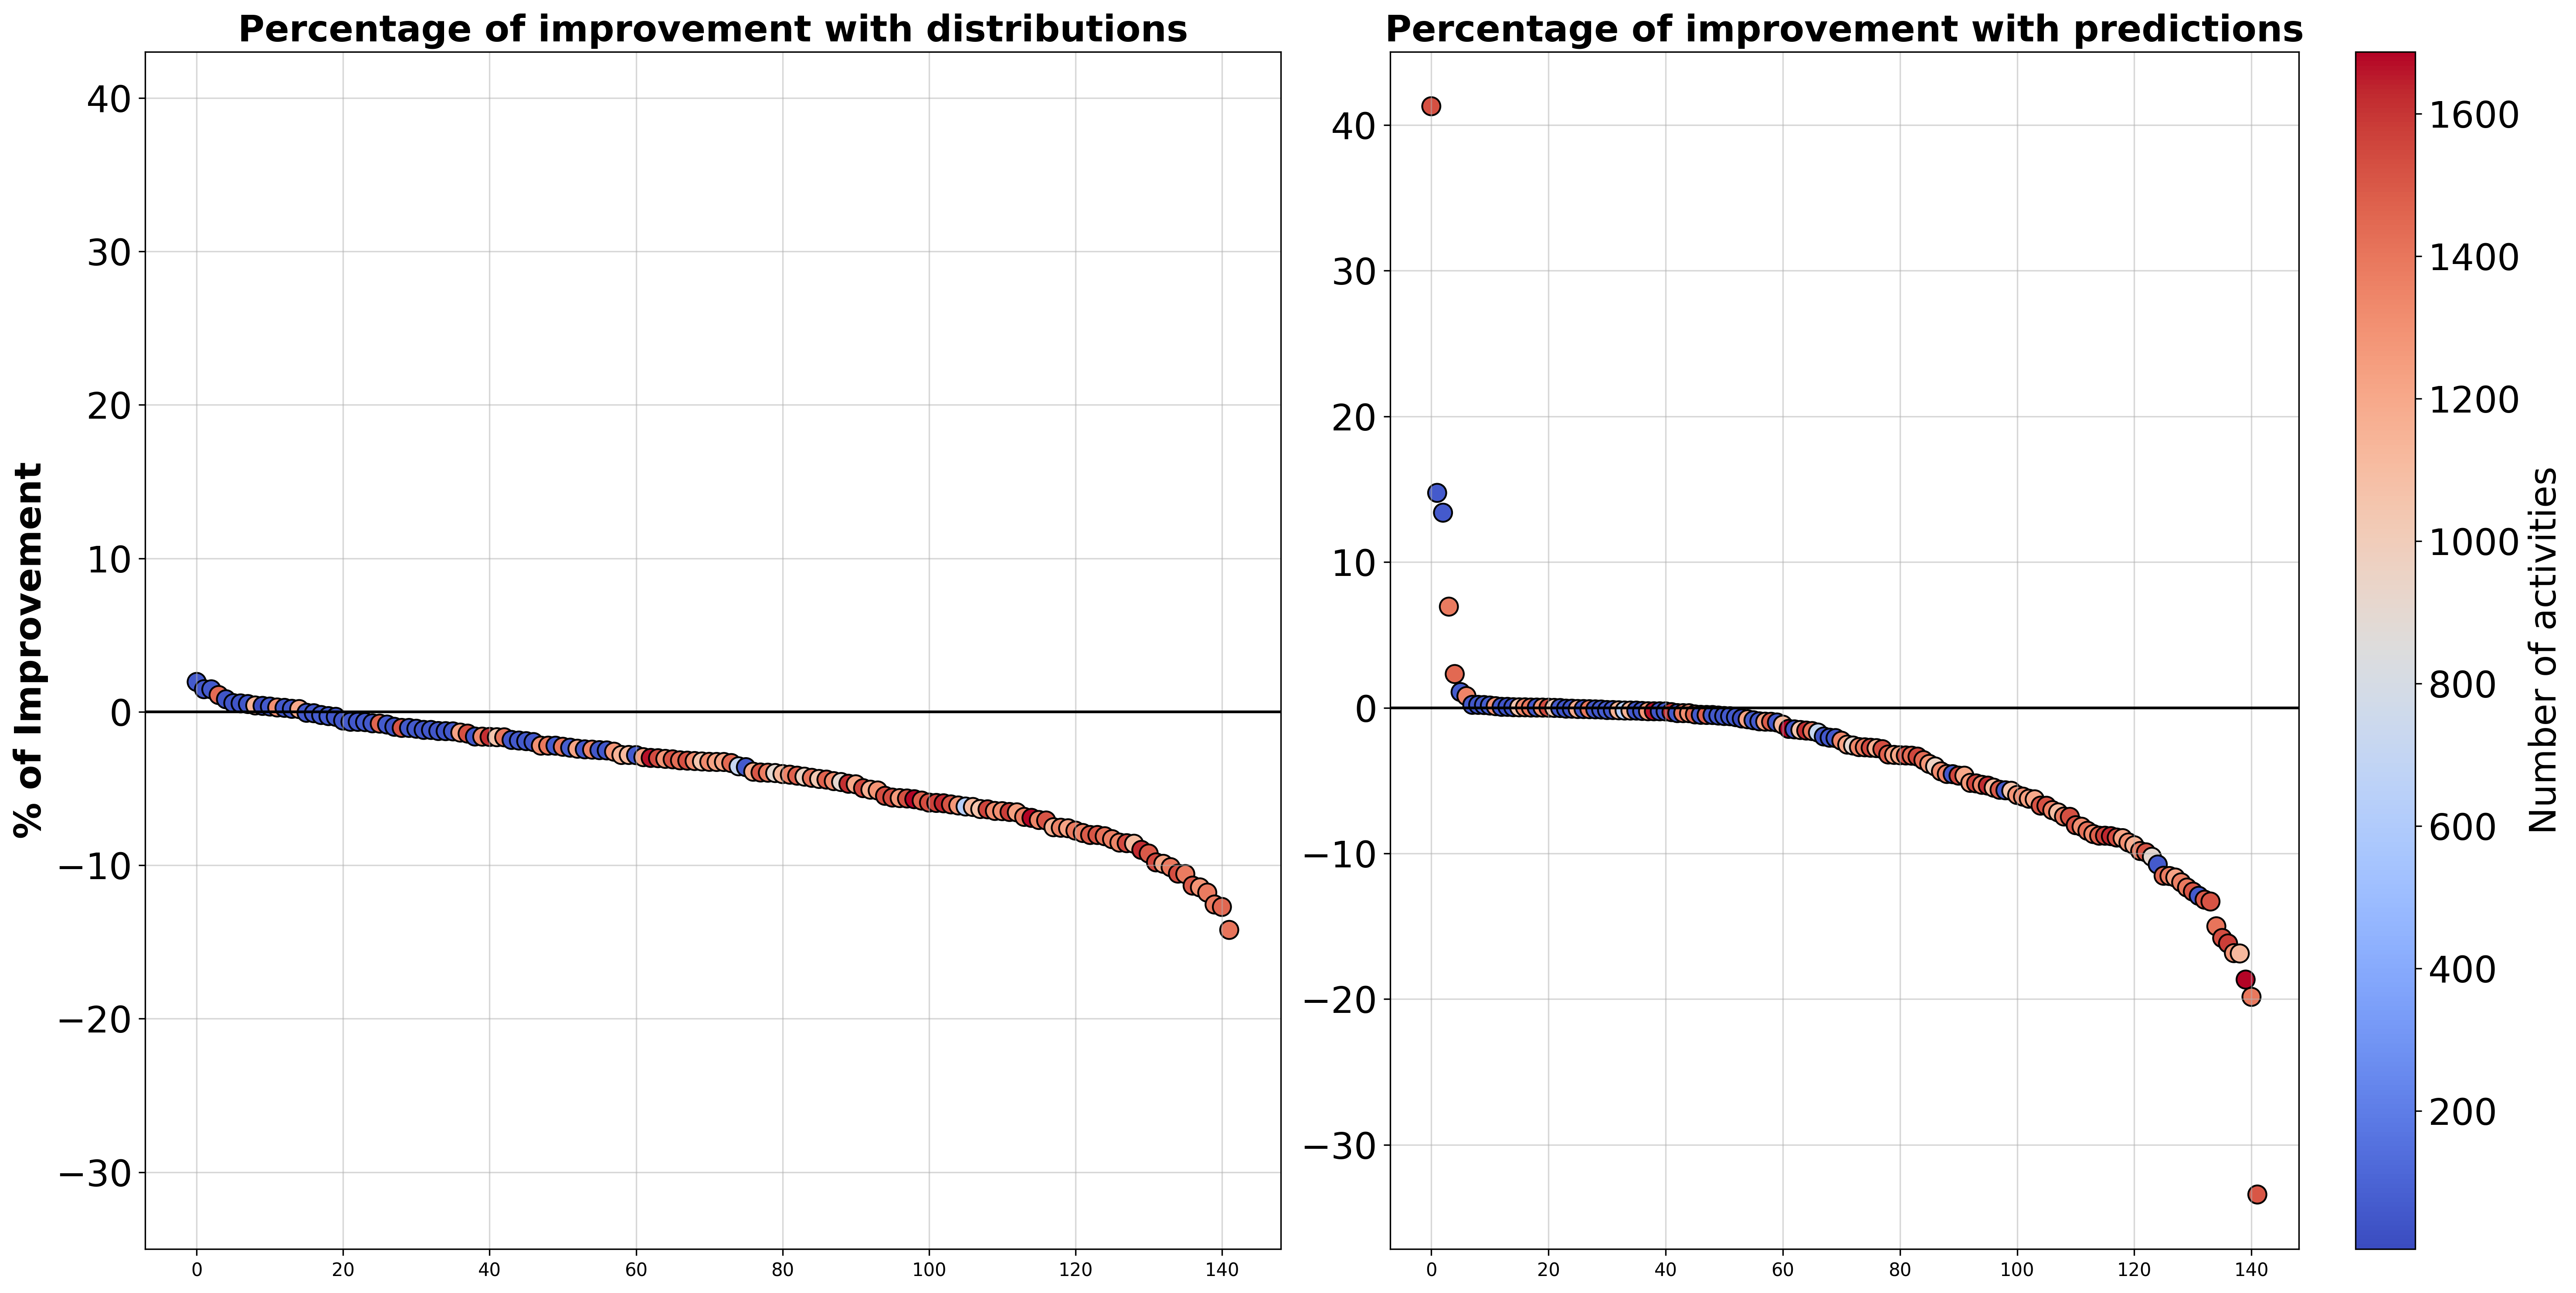
\includegraphics[width=\textwidth]{images/Imp.png}
\caption{}
\label{fig:improvements_real_dataset}
\end{figure*}



\subsection*{Technical material}

\subsubsection{Code for reproducing experiments} The \emph{IJCAI2025-Proactive-DataDriven-Scheduling-Business-Process} archive contains all the code used to reproduce the experiments, including the instructions for the environment set up. The instructions are reported in a Markdown file \emph{README.md}, detailing all the steps and commands for installation of all the packages detailed above.


\subsubsection*{Datasets}

The archive also contains the synthetic dataset, as well as the predictive models used for the second set of experiments. However, real data are not available due to privacy reasons.

\subsection{Additional results and plots}

In this section, we report other results and plots that extend Section~\ref{sec:evaluation}.  

\subsubsection{Synthetic data}

Table~\ref{tab:resultSynthetic_appendix} provides an extended overview of the first set of experiments (Table~\ref{tab:results_synthetic}). It reports, for each problem, the minimum makespan obtained with the CP solver ($M^*_{C}$), the probabilistic minimum makespan ($M^*_{\alpha}$), along with the corresponding mean ($\mu^*_{\alpha}$) and standard deviation ($\sigma^*_{\alpha}$). Moreover, 
Table~\ref{tab:resultSynthetic_appendix} presents the results for three additional problems of varying sizes: \{($20 \times 15$), \act{medium} ($30 \times 15$), and ($40 \times 20$)\}.

Table~\ref{tab:resultSynthetic_prediction_appendix} pertains to the second set of synthetic experiments, where predictive models are utilized to estimate the mean and the standard deviation of each activity in the problems. Similarly, Table~\ref{tab:resultSynthetic_prediction_appendix} provides the same additional information as Table~\ref{tab:resultSynthetic_appendix}, including $M^*_{C}$, $M^*_{\alpha}$, $\mu^*_{\alpha}$, and $\sigma^*_{\alpha}$, for the \act{small}, \act{medium}, and \act{big} problems.



